\documentclass[12pt]{ctexart}
\usepackage{amsmath, amssymb, enumitem, xcolor, graphicx, multicol}
\usepackage{floatrow}

\begin{document}

\section*{2024年全国甲卷理科数学真题}

\subsection*{一、选择题(每小题5分,共60分)}

\begin{enumerate}[label=\arabic*.]
    \item[\textcolor{red}{3}.] 若实数\( x,y \)满足约束条件
    \[
    \left\{
    \begin{aligned}
        4x - 3y &\geq 0 \\
        x - 2y - 2 &\leq 0 \\
        2x + 6y - 9 &\leq 0
    \end{aligned}
    \right.
    \]
    则\( z = x - 5y \)的最小值为()
    \begin{enumerate}[label=\Alph*.]
        \item \( 5 \)
        \item \( \dfrac{1}{2} \)
        \item 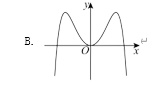
\includegraphics[width=0.3\textwidth]{cropped_0.jpg}
        \item 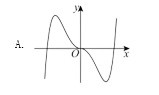
\includegraphics[width=0.3\textwidth]{cropped_1.jpg}
    \end{enumerate}
    
    \item[\textcolor{red}{7}.] 函数\( f(x) = -x^2 + (e^x - e^{-x})\sin x \)在区间\([-2.8,2.8]\)的大致图像为()
    \begin{enumerate}[label=\Alph*.]
        \item 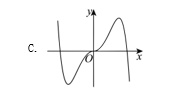
\includegraphics[width=0.3\textwidth]{cropped_2.jpg}
        \item 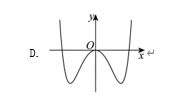
\includegraphics[width=0.3\textwidth]{cropped_3.jpg}
        \item 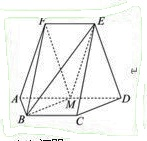
\includegraphics[width=0.3\textwidth]{cropped_4.jpg}
        \item \includegraphics[width=0.3\textwidth]{cropped_5.jpg}
    \end{enumerate}
    
    \item[\textcolor{red}{8}.] 已知\( \dfrac{\cos\alpha}{\cos\alpha - \sin\alpha} = \sqrt{3} \),则\( \tan\left(\alpha + \dfrac{\pi}{4}\right) = \)()
    \begin{enumerate}[label=\Alph*.]
        \item \( 2\sqrt{3} + 1 \)
        \item \( 2\sqrt{3} - 1 \)
        \item \( \dfrac{\sqrt{3}}{2} \)
        \item \( 1 - \sqrt{3} \)
    \end{enumerate}
    
    \item[\textcolor{red}{11}.] 在\( \triangle ABC \)中,内角\( A,B,C \)所对边分别为\( a,b,c \),若\( B = \dfrac{\pi}{3} \),\( b^2 = \dfrac{9}{4}ac \),则\( \sin A + \sin C = \)()
    \begin{enumerate}[label=\Alph*.]
        \item \( \dfrac{3}{2} \)
        \item \( \sqrt{2} \)
        \item \( \dfrac{\sqrt{7}}{2} \)
        \item \( \dfrac{\sqrt{3}}{2} \)
    \end{enumerate}
\end{enumerate}

\subsection*{三、解答题(共70分)}

\subsubsection*{(一) 必考题(共60分)}

\begin{enumerate}[resume*]
    \item[\textcolor{red}{17}.] 某工厂进行生产线智能化升级改造,升级改造后,从该工厂甲、乙两个车间的产品中随机抽取150件进行检验,数据如下:
    \begin{table}[H]
        \centering
        \begin{tabular}{c|c|c|c|c}
            \hline
            & 优级品 & 合格品 & 不合格品 & 总计 \\
            \hline
            甲车间 & 26 & 24 & 0 & 50 \\
            \hline
            乙车间 & 70 & 28 & 2 & 100 \\
            \hline
            总计 & 96 & 52 & 2 & 150 \\
            \hline
        \end{tabular}
    \end{table}
    (1)填写下列列联表:
    \begin{table}[H]
        \centering
        \begin{tabular}{c|c|c|c}
            \hline
            & 优级品 & 非优级品 & 总计 \\
            \hline
            甲车间 & & & \\
            \hline
            乙车间 & & & \\
            \hline
        \end{tabular}
    \end{table}
    能否有95\%的把握认为甲、乙两车间产品的优级品率存在差异?能否有99\%的把握认为甲、乙两车间产品的优级品率存在差异?
    
    (2)已知升级改造前该工厂产品的优级品率\( p = 0.5 \),设\( P \)为升级改造后抽取的\( n \)件产品的优级品率。如果\( P > p + 1.65\sqrt{\dfrac{p(1-p)}{n}} \),则认为该工厂产品的优级品率提高了。根据抽取的150件产品的数据,能否认为生产线智能化升级改造后,该工厂产品的优级品率提高了?
\end{enumerate}

\subsubsection*{其他解答题}

\begin{enumerate}[resume*]
    \item[\textcolor{red}{19}.] 如图,在以\( A,B,C,D,E,F \)为顶点的五面体中,四边形\( ABCD \)与四边形\( ADEF \)均为等腰梯形,\( BC \parallel AD \),\( EF \parallel AD \),\( AD = 4 \),\( AB = BC = EF = 2 \),\( ED = \sqrt{10} \),\( FB = 2\sqrt{3} \),\( M \)为\( AD \)的中点。
    \begin{enumerate}[label=(\arabic*)]
        \item 证明:\( BM \parallel \)平面\( CDE \)
        \item 求二面角\( F-BM-E \)的正弦值
    \end{enumerate}
    \begin{figure}[H]
        \centering
        \includegraphics[width=0.5\textwidth]{cropped_6.jpg}
    \end{figure}
    
    \item[\textcolor{red}{20}.] 设椭圆\( C:\dfrac{x^2}{a^2} + \dfrac{y^2}{b^2} = 1(a > b > 0) \)的右焦点为\( F \),点\( M\left(\dfrac{1}{3}, \dfrac{3}{2}\right) \)在\( C \)上,且\( MF \perp x \)轴。
    \begin{enumerate}[label=(\arabic*)]
        \item 求\( C \)的方程
        \item 过点\( P(4,0) \)的直线与\( C \)交于\( A,B \)两点,\( N \)为线段\( FP \)的中点,直线\( NB \)交直线\( MF \)于点\( Q \),证明:\( AQ \perp y \)轴
    \end{enumerate}
\end{enumerate}

\subsection*{底部引用图片}
\begin{figure}[H]
    \centering
    \begin{minipage}{0.3\textwidth}
        \includegraphics[width=\textwidth]{cropped_6.jpg}
    \end{minipage}
    \hfill
    \begin{minipage}{0.3\textwidth}
        \includegraphics[width=\textwidth]{cropped_7.jpg}
    \end{minipage}
    \hfill
    \begin{minipage}{0.3\textwidth}
        \includegraphics[width=\textwidth]{cropped_8.jpg}
    \end{minipage}
    \caption{底部引用图片}
\end{figure}

\end{document}